\section[Profilowanie]{Profilowanie}\label{sec:profiling} 

\subsection{Parametry uruchomienia}

W celu weryfikacji i porównania możliwości \pythonpic{} na jego podstawie
utworzono uproszczony, analogiczny kod w C++ (``CPIC''), również dostępny na platformie
GitHub~\footnote{\url{https://github.com/StanczakDominik/CPIC}} i oparty o bibliotekę macierzową Eigen~\cite{eigen}.
Porównano jego rezultaty z \pythonpic{}, osiągając dobrą zgodność.


Na potrzeby wykonania profilowania wydajności kodu przygotowano w obu wersjach
programu uproszczoną wersję symulacji z laserem z rozdziału~\ref{sec:verification}.
Uproszczenie polega na rozmieszczeniu cząstek w jednorodnej bryle na środku symulacji.
Profilowanie przeprowadzono przez 1000 iteracji programu dla zmiennej liczby cząstek i ustalonej liczby 1000
komórek Eulera, w przypadku polaryzacji liniowej i mocy lasera $10^{21} W/m^2$.
Wartości fizycznych zmiennych wykorzystane do przeprowadzenia profilowania są dostępne w repozytorium CPIC.

Profilowanie przeprowadzono na komputerze o procesorze 
Intel Core 4 Quad 6600 3.0GHz i 4GB RAM, wykorzystując następujące wersje
oprogramowania i bibliotek obliczeniowych:
\begin{itemize}
\itemi{} Python 3.6.2
\itemi{} Numpy 1.13.3
\itemi{} Numba 0.34.0
\itemi{} SciPy 0.19.1
\itemi{} gcc 7.2.0
\itemi{} Eigen 3.3.4
\end{itemize}

Dla \pythonpic{} przeprowadzono testy w czystym Pythonie (opartym na wysokopoziomowym zastosowaniu Numpy)
i w wersji próbującej optymalizować najintensywniejsze fragmenty obliczeń (relatywistyczny integrator Borysa
oraz algorytm depozycji ładunku) poprzez kompilację JIT z wykorzystaniem Numba. Należy zauważyć, że ze względu
na wykorzystany wysokopoziomy paradygmat obliczeń nie udało się przekompilować kodu z wykorzystaniem
wydajniejszej opcji \code{nopython} i pozostano przy kompilacji ``domyślnej'' w tzw.\ trybie obiektowym.

Dla CPIC testy przeprowadzono w trzech wariacjach, bez flag optymalizacyjnych oraz z flagami \code{-O}, \code{-O2}.
Pominięto niektóre wyniki symulacji z powodu bliżej niezidentyfikowanych błędów kończących symulację w niepokojąco
krótkim czasie. Błędów tych nie udało się zlokalizować, ale pozostałe symulacje zwracają wyniki zgodne z oczekiwaniami.

We wszystkich przypadkach pominięto zapis danych symulacyjnych do pliku oraz
inicjalizację warunków początkowych, mierząc wydajność samych obliczeń.

\subsection{Wyniki}

\begin{table}[H]
\centering
\footnotesize
\label{table:runtime}
\begin{tabular}{llllll}
\toprule
{} & Python & Python (JIT) & C bez flag &  C -O & C -O2 \\
liczba cząstek &        &              &            &       &       \\
\midrule
100            &  15.89 &        22.27 &       3.09 &  0.10 &  0.16 \\
200            &  14.39 &        20.51 &       6.28 &  0.27 &  0.26 \\
500            &  17.17 &        23.44 &         -- &    -- &    -- \\
750            &     -- &           -- &       4.65 &  0.50 &  0.98 \\
1000           &  21.71 &        28.04 &         -- &    -- &    -- \\
1750           &     -- &           -- &      42.46 &  1.06 &    -- \\
2000           &  28.87 &        36.10 &      49.98 &  1.22 &  2.33 \\
2500           &     -- &           -- &      67.72 &  1.55 &  2.82 \\
5000           &  49.72 &        57.16 &     132.50 &  3.14 &  2.11 \\
10000          &  86.44 &        96.94 &     244.85 &  6.37 &  4.18 \\
20000          & 210.88 &       181.14 &     479.70 & 24.35 &  8.40 \\
50000          & 659.10 &       613.81 &    1617.79 & 64.69 & 21.51 \\
\bottomrule
\end{tabular}

\caption{Czas działania symulacji, w sekundach.}
\end{table}

\begin{figure}[h!]
  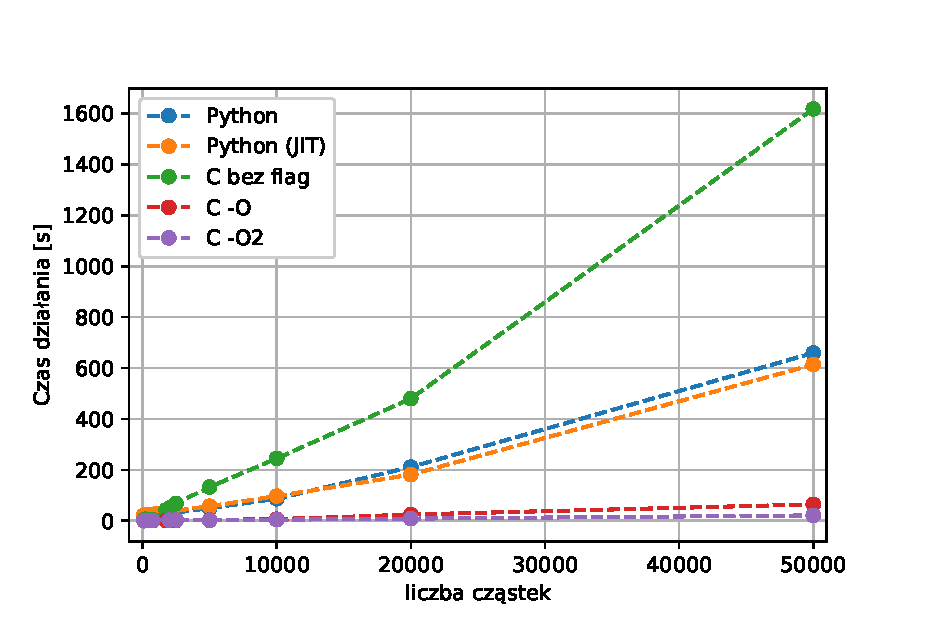
\includegraphics[width=\textwidth]{Images/runtimes}
  \caption{Czas działania symulacji.}\label{fig:runtime}
\end{figure}

\begin{figure}[h!]
  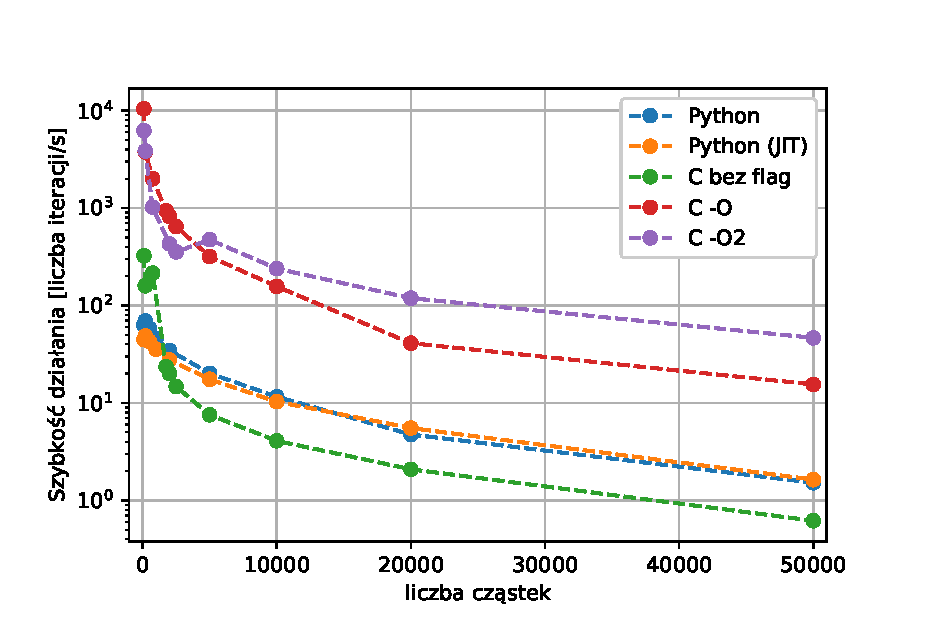
\includegraphics[width=\textwidth]{Images/speeds}
  \caption{Szybkość działania symulacji}\label{fig:runspeed}
\end{figure}
